	\chapter{Results and discussion}

The survey of Andromeda Galaxy according to [15], gives us the rotation curve measured out to $38$ kpc, showing a peak at $340$ km s$^{-1}$ , a dip at $202$ km s$^{-1}$ around $4$ kpc, two distinct flat parts at $264$ km s$^{-1}$  and $230$ km s$^{-1}$ and an increase to $275$  km s $^{-1}$ in the outermost regions \cite{observed}.
 
 Regenerating the curve, using the program in section $2.3$, the observed rotation curve of M31 is obtained.

\begin{figure} [h]
\centering
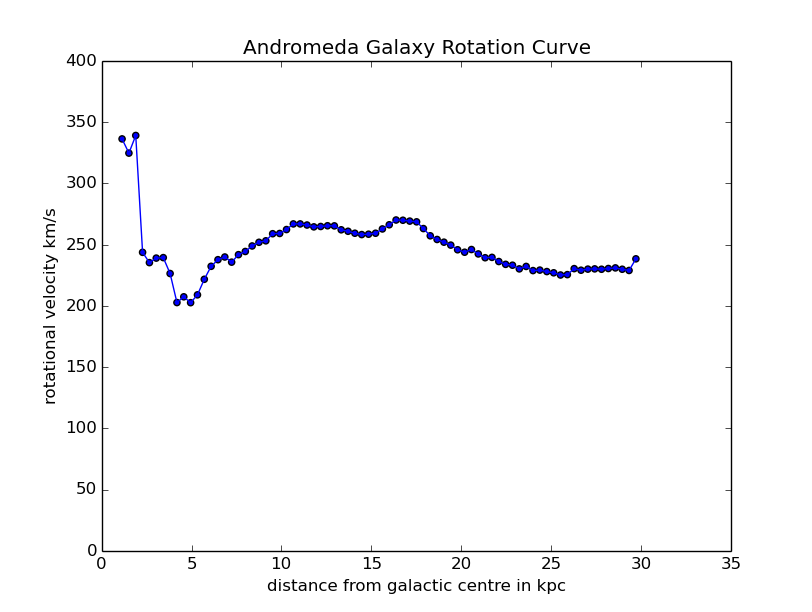
\includegraphics[scale=0.5]{rotcurve}
\caption{Observed Rotation Curve for Andromeda Galaxy}
\end{figure}

\section{Optimized Rotation Curve}

The rotation curve obtained from the data, that was calculated using Image Analysis as explained in section 2.2.1  was optimized, and the resulting plot is:

\begin{figure} [h]
\centering
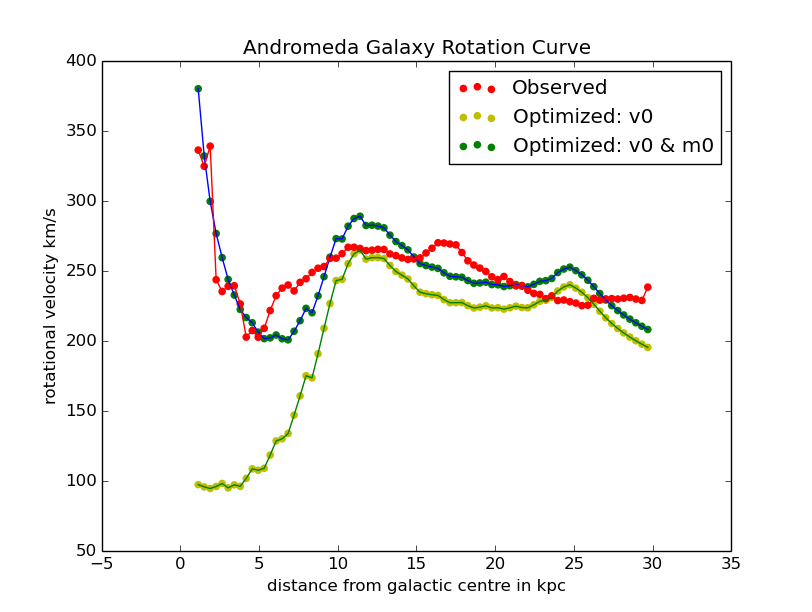
\includegraphics[scale=0.5]{best}
\caption{Rotation Curve for Andromeda Galaxy}
\end{figure}

\section{Need for Optimization}

The rotation curve obtained by using the precalculated data, is to be achieved by the data calculated by image analysis. When we plot the curve from our calculated data, it gives us an irregular pattern, which demands that there must be some fitting done for it. After which we optimize the graph to a certain velocity and the optimization function gives us the value of velocity. From Figure $2.8$ we find the curve described as \textit{optimized for velocity} \textbf{$v_{0}$} is in some accordance with the observed rotation curve, but it still requires some modification in the region near the origin. For that purpose, we optimize the curve for masses also, and similarly, the funtion gives us optimized value of mass \textbf{$m_{0}$}. 

The values of $v_{0}$ and $m_{0}$ are found out to be;

$v_{0} = 55802.2453 $         

$m_{0} = 1473818.3329 $

with standard deviations of ;

$\triangle v =  4.67802922e+05$

$\triangle m = 7.79892330e+09 $

The units for these values are not defined, as they could be explained by any multiplicative factor in the units of velocity and masses. 